% Universidade Federal do Rio Grande do Norte
% Programa de Pos-Graduacao em Engenharia Eletrica e de Computacao
% Lista 1 - Questao 1
% Autores: Anna Giselle Camara Dantas Ribeiro
%          Cristiano Gurgel de Castro
%          Diogo Leite Reboucas
%          Thiago Medeiros Barros

% Revisado em 15/06/2010 12:45 por crisgc
%   - Falta completar os itens c) a e)

\chapter*{Questão 1}
% Enunciado
\noindent {\it Considere o sistema:}

\begin{equation}\nonumber
G(s) = \frac{Y(s)}{U(s)} = \frac{0.5}{(s+0.5)(s+1)}
\end{equation}

{\it Pede-se:}

\begin{itemize}
    \item[a)] {\it Discretize o sistema com um período de amostragem de 0.2 s}
    \item[b)] {\it Obtenha o modelo FSR (resposta ao degrau Truncada) do sistema
              considerando $N = 10$}
    \item[c)] {\it Calcule a resposta do sistema a uma entrada qualquer
              utilizando a equação obtida no item (b) e compare com o seu valor 
              exato}
    \item[d)] {\it Obtenha a expressão do sinal de controle do controlador DMC,
              considerando $NY = NU = 5$ e $\lambda = 0.8$}
    \item[e)] {\it Simule no \Matlab (ou \Scilab) o sistema com o controlador
              projetado no item (d)}
\end{itemize}

\vspace{0.5cm}

\noindent{\bf Resolução:}

\vspace{0.25cm}

\section*{Item A}
Uma maneira simples de realizar a discretização de funções de transferência é
utilizar o método da invariância ao degrau, no qual a idéia é a de se utilizar
um Segurador de Ordem Zero ({\it Zero Order Holder} -- ZOH) para aproximar a
função de transferência $G(s)$ de $G(z)$. Matematicamente, a discretização de
uma função de transferência analógica $G(s)$ por tal método é dada por:

\begin{equation}\label{eq:Gzoh}
G_{\text{ZOH}}(z) = 
G(z) = (1 - z^{-1})
       \zadeh\chave{\ilaplace\left.\colchete{\frac{G(s)}{s}}\right|_{t = nT}}
\end{equation}

\noindent em que $\zadeh$ corresponde à {\it Transformada Z}, $\ilaplace$ à {\it
Transformada Inversa de Laplace} e, para $t = nT$, $T$ corresponde ao período de
amostragem e $z = e^{-sT}$. Então, para a função de transferência $G(s)$ dada no
enunciado:

\begin{equation}\label{eq:Gs_s}
\frac{G(s)}{s} = \frac{0.5}{s(s+0.5)(s+1)}
\end{equation}

Expandindo a Eq. \ref{eq:Gs_s} em frações parciais, tem-se que:

\begin{eqnarray}\label{eq:frac_parc}
\frac{G(s)}{s} & = & \colchete{\frac{0.5}{s(s+0.5)(s+1)}}\nonumber\\
& = & \frac{A}{s} + \frac{B}{s+0.5} + \frac{C}{s+1}\nonumber\\
\end{eqnarray}

Mas,

\begin{eqnarray}
A & = & \left.\frac{0.5}{(s+0.5)(s+1)}\right|_{s = 0} = \frac{0.5}{0.5} = 
                                                    1\nonumber\\
B & = & \left.\frac{0.5}{s(s+1)}\right|_{s = -0.5} = \frac{0.5}{-0.25} = 
                                                 -2\nonumber\\
C & = & \left.\frac{0.5}{s(s+0.5)}\right|_{s = -1} = \frac{0.5}{0.5} = 
                                                     1\nonumber
\end{eqnarray}

Então, aplicando então a transformada inversa de Laplace, tem-se que:

\begin{eqnarray}
\ilaplace\colchete{\frac{G(s)}{s}}
& = & \ilaplace\colchete{\frac{1}{s} - 
                         2\frac{1}{s+0.5} + 
                         \frac{1}{s+1}}\nonumber\\
& = & \ilaplace\colchete{\frac{1}{s}} - 
      2\ilaplace\colchete{\frac{1}{s+0.5}} + 
      \ilaplace\colchete{\frac{1}{s+1}}\nonumber\\
& = & 1 - 2e^{-0.5t} + e^{-t}\label{eq:ilaplace}
\end{eqnarray}

Substituindo a Eq. \ref{eq:ilaplace} na Eq. \ref{eq:Gzoh} quando $t = nT$,
tem-se:

\begin{eqnarray}
G(z) & = & (1 - z^{-1})
           \zadeh\chave{\ilaplace\left.\colchete{\frac{G(s)}{s}}
                                  \right|_{t = nT}}\nonumber\\
& = & \parent{\frac{z-1}{z}}
      \zadeh\colchete{1 - 2e^{-0.5nT} + e^{-nT}}\nonumber\\
& = & \frac{z-1}{z}\chave{\zadeh\colchete{1} - 
                          2\zadeh\colchete{e^{-0.5nT}} + 
                          \zadeh\colchete{e^{-nT}}}\nonumber\\
& = & \frac{z-1}{z}\parent{\frac{z}{z-1} - 
                           2\frac{z}{z-e^{-0.5nT}} + 
                           \frac{z}{z - e^{-nT}} }\nonumber\\
& = & \frac{z-1}{z-1} - 
      2\frac{z-1}{z-e^{-0.5nT}} + 
      \frac{z-1}{z - e^{-nT}}\nonumber\\
\end{eqnarray}

Desconsideranto o termo $n$, referente a $n$-ésima amostra em $nT$ e
substituindo $T = 0.2$, tem-se:

\begin{eqnarray}
G(z) & = & \frac{z-1}{z-1} - 
           2\frac{z-1}{z-e^{-0.5 \cdotp 0.2}} + 
           \frac{z-1}{z-e^{-0.2}}\nonumber\\
& = & 1 - 
      2\frac{z-1}{z-\underbrace{0.9048}_{\alpha}} + 
      \frac{z-1}{z-\underbrace{0.8187}_{\beta}}\nonumber\\
& = & \frac{1(z-\alpha)(z-\beta)-2(z-1)(z-\beta)+(z-1)(z-\alpha)}
           {(z-\alpha)(z-\beta)}\nonumber\\
& = & \frac{(-2\alpha + \beta + 1)z + (\alpha\beta - 2\beta + \alpha)}
           {z^2 - (\alpha+\beta)z + \alpha\beta}\nonumber\\
& = & \frac{0.0091z + 0.0082}{z^2 - 1.7235z + 0.7408}
\end{eqnarray}

Sabendo que a função de transferência de um sistema é definida como sendo a {\it
Transformada de Laplace} da resposta ao impulso com condições iniciais nulas, e
que seu equivalente em $\zadeh$ possui as mesmas características, então:

\begin{eqnarray}
G(z) = \frac{Y(z)}{U(z)} & = & \frac{0.0091z + 0.0082}
                                    {z^2 - 1.7235z + 0.7408}\nonumber\\
Y(z)(z^2 - 1.7235z + 0.7408) & = & U(z)(0.0091z + 0.0082)\nonumber\\
z^2Y(z) - 1.7235zY(z) + 0.7408Y(z) & = & 0.0091zU(z) +
                                        0.0082U(z)\label{eq:sist_z}
\end{eqnarray}

Aplicando a transformada $\zadeh$ inversa na Eq. \ref{eq:sist_z}, tem-se:

\begin{eqnarray}
z^2Y(z) - 1.7235zY(z) + 0.7408Y(z) & = & 0.0091zU(z) + 0.0082U(z)
\quad\stackrel{\izadeh}{\Longrightarrow}\quad\nonumber\\
\stackrel{\izadeh}{\Longrightarrow}\quad
y(k+2) - 1.7235y(k+1) + 0.7408k(k) & = & 
0.0091u(k+1) + 0.0082u(k)\nonumber\\
y(k) - 1.7235y(k-1) + 0.7408k(k-2) & = & 
0.0091u(k-1) + 0.0082u(k-2)\label{eq:yk}
\end{eqnarray}

O resultado obtido na Eq. \ref{eq:sist_z} pode ser confirmado fazendo uso da
função {\tt c2d} do \Matlab, conforme {\it
script} desenvolvido, mostrado no Apêndice \ref{ap:q1_a}.

\section*{Item B}
Para \citeasnoun{santos:2007}, a modelagem de um processo dinâmico consiste em
obter um modelo matemático capaz de representar adequadamente suas
características de interesse. Tal recurso se torna muitas vezes fundamental
quando o processo real apresenta restrições de ordem operacional,
econômico-financeira ou de segurança.

O modelo de um sistema pode ser obtido, basicamente, de duas formas: a partir
das equações que descrevem sua dinâmica ({\it modelagem fenomenológica}) ou a
partir da medição de dados de entrada e saída. Dentre os modelos que levam em
consideração essa relação entrada/saída do sistema, existem os modelos {\bf
paramétricos} e os modelos {\bf não paramétricos}.

Os modelos paramétricos correspondem àqueles que apresentam parâmetros
característicos. Tais parâmetros são os coeficientes de uma equação a diferenças
ou de uma função de transferência discreta do sistema. Já os modelos não
paramétricos representam a dinâmica do processo através dos coeficientes da
resposta ao impulso ({\it modelos} FIR -- {\it Finite Impulse Response}) ou da
resposta ao degrau ({\it modelos} ISR -- {\it Infinite Step Response} {\it e}
FSR -- {\it Finite Step Response}). \cite{santos:2007}

O modelo matemático baseado na resposta ao degrau representa o processo com um
número infinito de termos que correspondem aos coeficientes da resposta ao
degrau do sistema (ISR). Para sistemas estáveis, esses coeficientes tendem,
assintoticamente, para um valor constante $h_s$, conforme Fig. \ref{fig:isr}.

\begin{figure}[htb]
\centering
    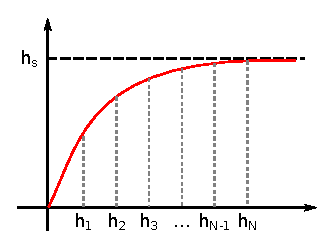
\includegraphics[width=0.35\textwidth]{imgs/questao1/isr}
    \caption{Exemplo de saída do sistema para o modelo ISR.}
    \label{fig:isr}
\end{figure}

O modelo FSR corresponde ao modelo de resposta ao degrau limitando o número de
coeficientes a um valor $N$. Tal modelo, também conhecido como modelo de
resposta ao degrau truncada, tem fundamentação convolutiva para relacionar a
entrada com a saída do sistema. Vale observar que nesse modelo o ruído não é
levado em consideração. A saída do processo no modelo FSR é dada pela Eq.
\ref{eq:saida_fsr}

\begin{equation}\label{eq:saida_fsr}
y(k) = \sum_{i=1}^N h_i\Delta u(k-i)
\end{equation}

Para o valor de $N = 10$ dado no enunciado da questão, tem-se

\begin{eqnarray}
y(10) & = & h_1\Delta u(9) + h_2\Delta u(8) + h_3\Delta u(7) + h_4\Delta u(6) +
            h_5\Delta u(5) + \nonumber\\ 
      & + & h_6\Delta u(4) + h_7\Delta u(3) + h_8\Delta u(2) + h_9\Delta u(1) + 
            h_{10}\Delta u(0)\nonumber
\end{eqnarray}

Considerando $\hat{y}(k)$ como a saída dada pela Eq. \ref{eq:yk}, então:

\begin{eqnarray}
y(10) & = & \hat{y}(1)[u(9)-u(8)] + 
            \hat{y}(2)[u(8)-u(7)] + 
            \hat{y}(3)[u(7)-u(6)] + \nonumber\\
      & + & \hat{y}(4)[u(6)-u(5)] +
            \hat{y}(5)[u(5)-u(4)] +
            \hat{y}(6)[u(4)-u(3)] + \nonumber\\
      & + & \hat{y}(7)[u(3)-u(2)] +
            \hat{y}(8)[u(2)-u(1)] +
            \hat{y}(9)[u(1)-u(0)] + \nonumber\\
      & + & \hat{y}(10)[u(0)-\cancel{u(-1)}] \nonumber
\end{eqnarray}

Para uma entrada degrau, $u(k) - u(k-1) = 0$, portanto:

\begin{equation}
y(10) = \hat{y}(10)u(0) = 
        [1.7235y(9) - 0.7408y(8) + 0.0091u(9) + 0.0082u(8)]u(0)
\end{equation}

\section*{Item C}
Para efeitos comparativos foi utilizada uma entrada degrau, cujos resultados
podem ser observados nas Figs. \ref{fig:item_c_10} a \ref{fig:item_c_100} para
valores de $N = 10\text{,}\ 25\text{,}\ 50\ \text{e}\ 100$.

\begin{figure}[H]
\centering
    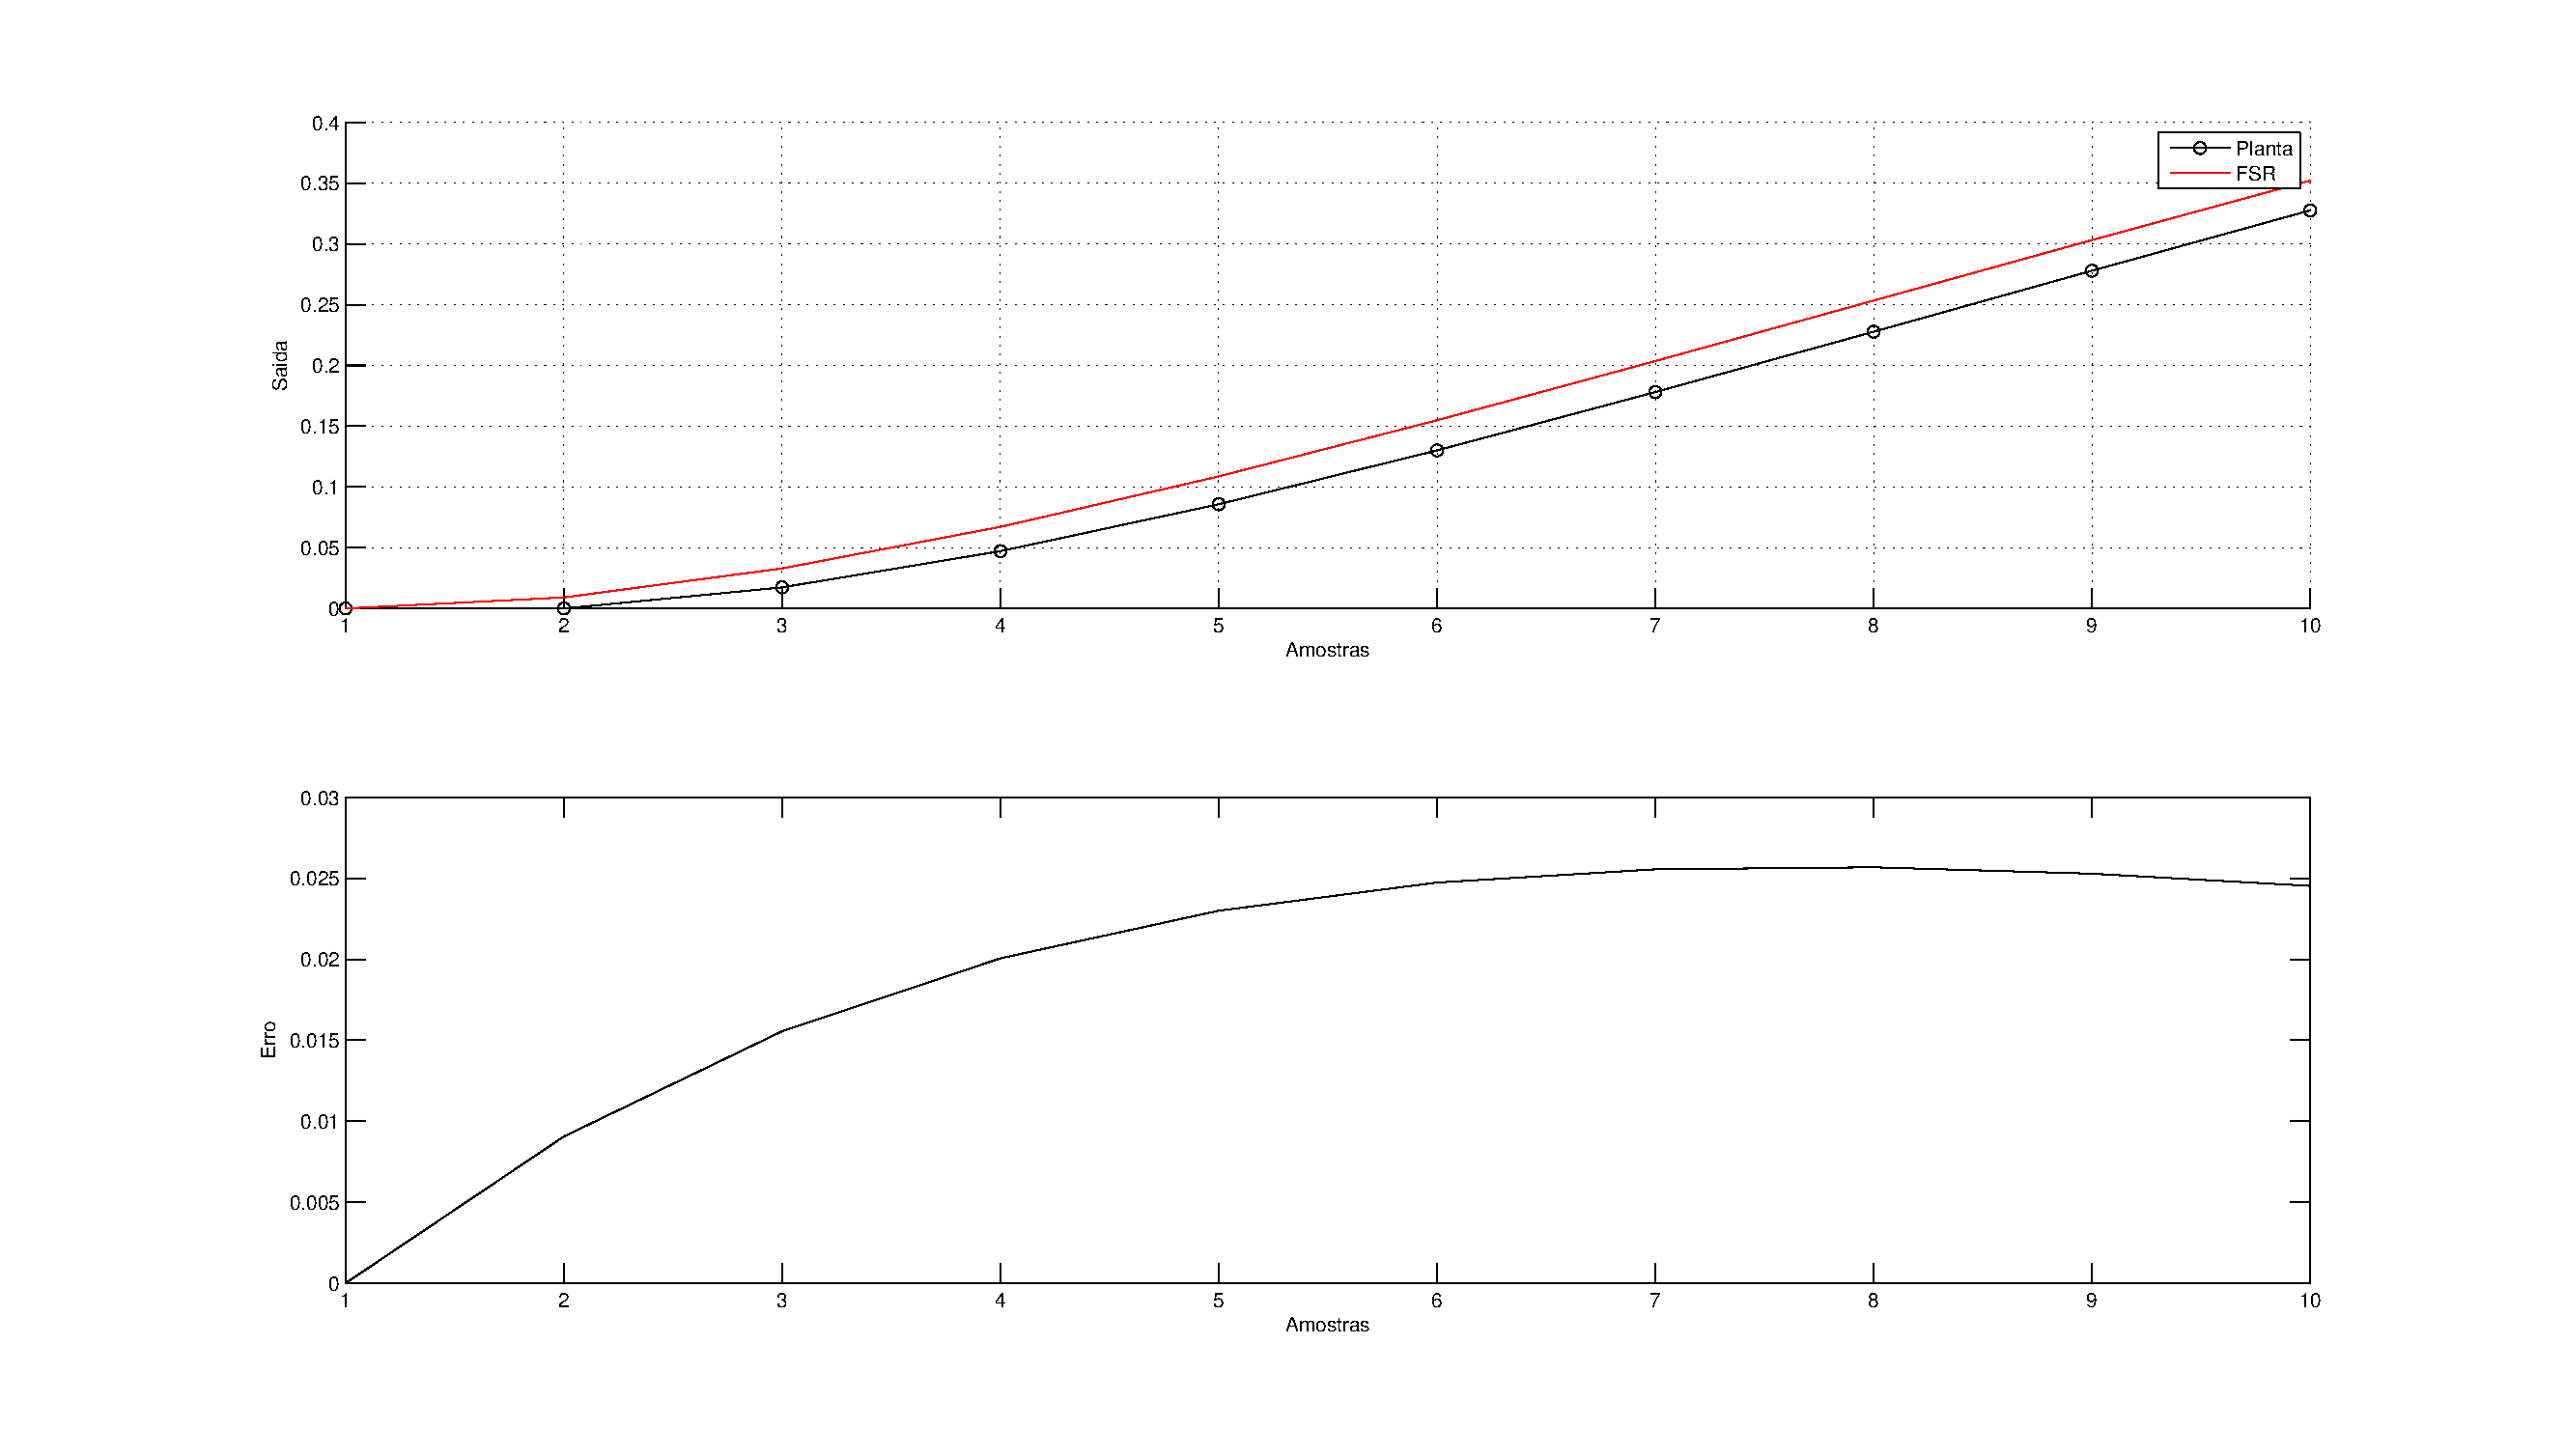
\includegraphics[width=0.95\textwidth]{imgs/questao1/item_c_N_10}
    \caption{Comparação realizada com $N = 10$.}
    \label{fig:item_c_10}
\end{figure}
    
\begin{figure}[htb]
\centering
    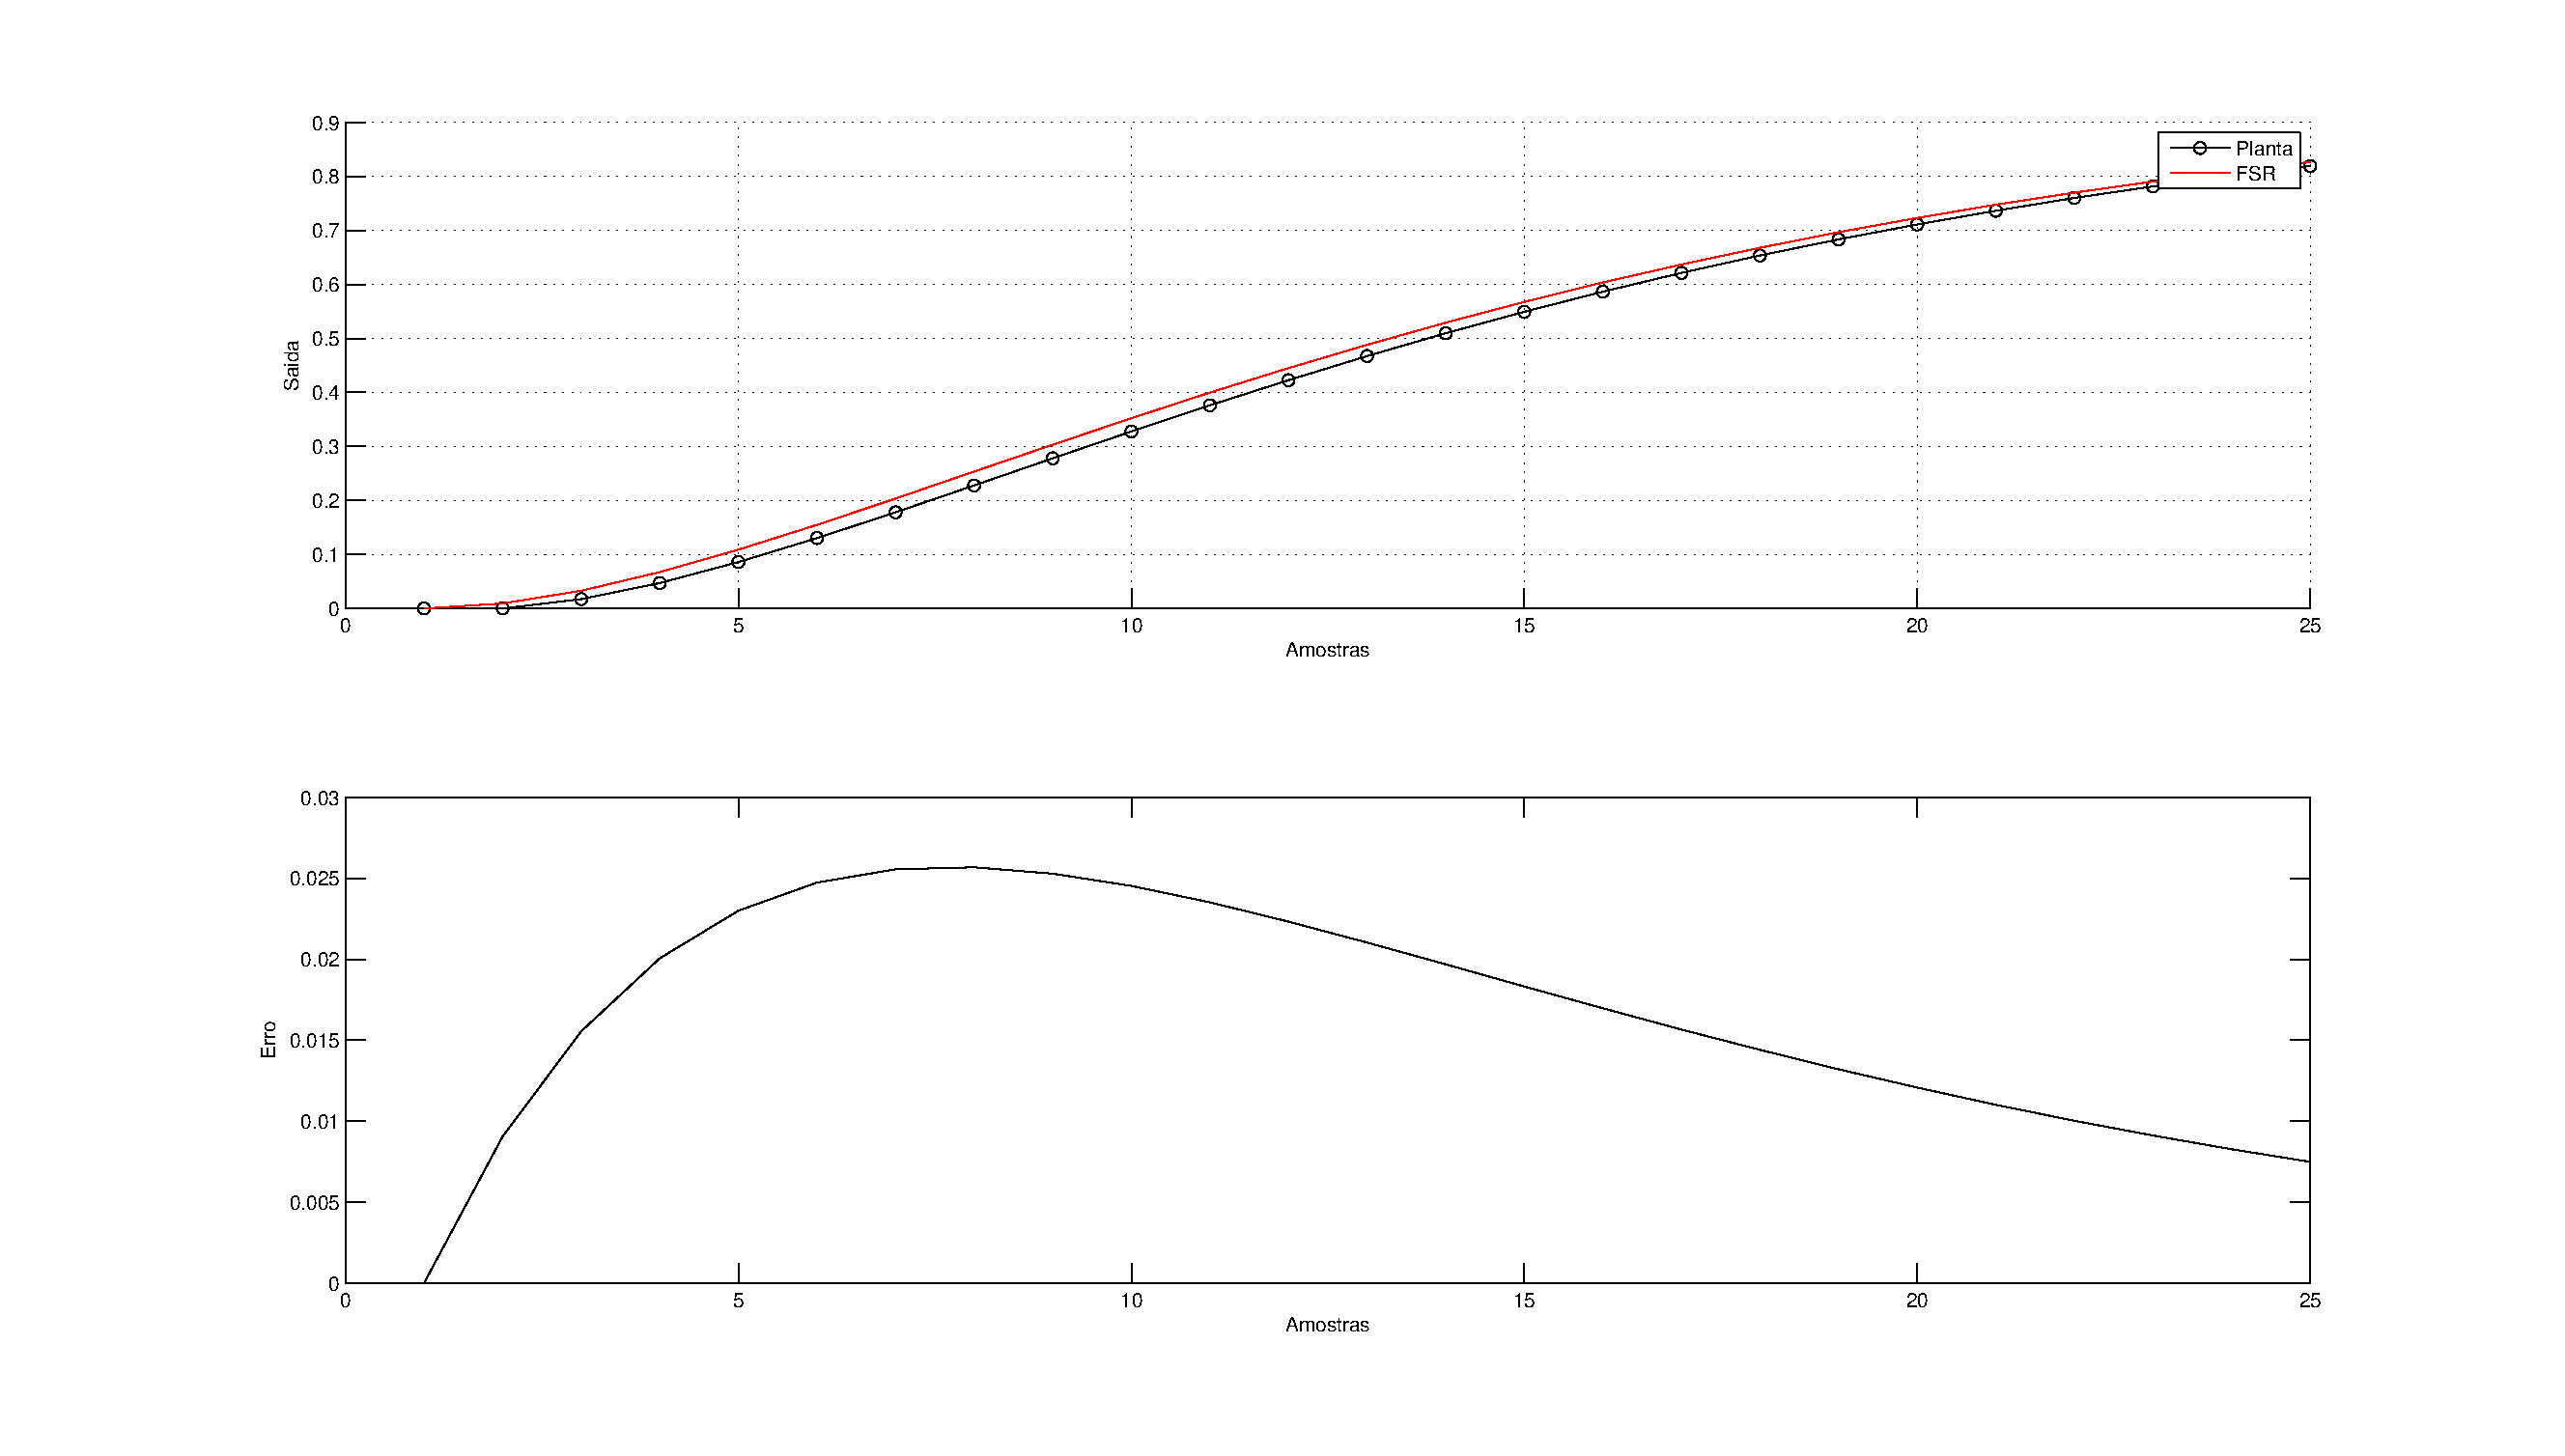
\includegraphics[width=0.95\textwidth]{imgs/questao1/item_c_N_25}
    \caption{Comparação realizada com $N = 25$.}
    \label{fig:item_c_25}
\end{figure}

\begin{figure}[htb]
\centering
    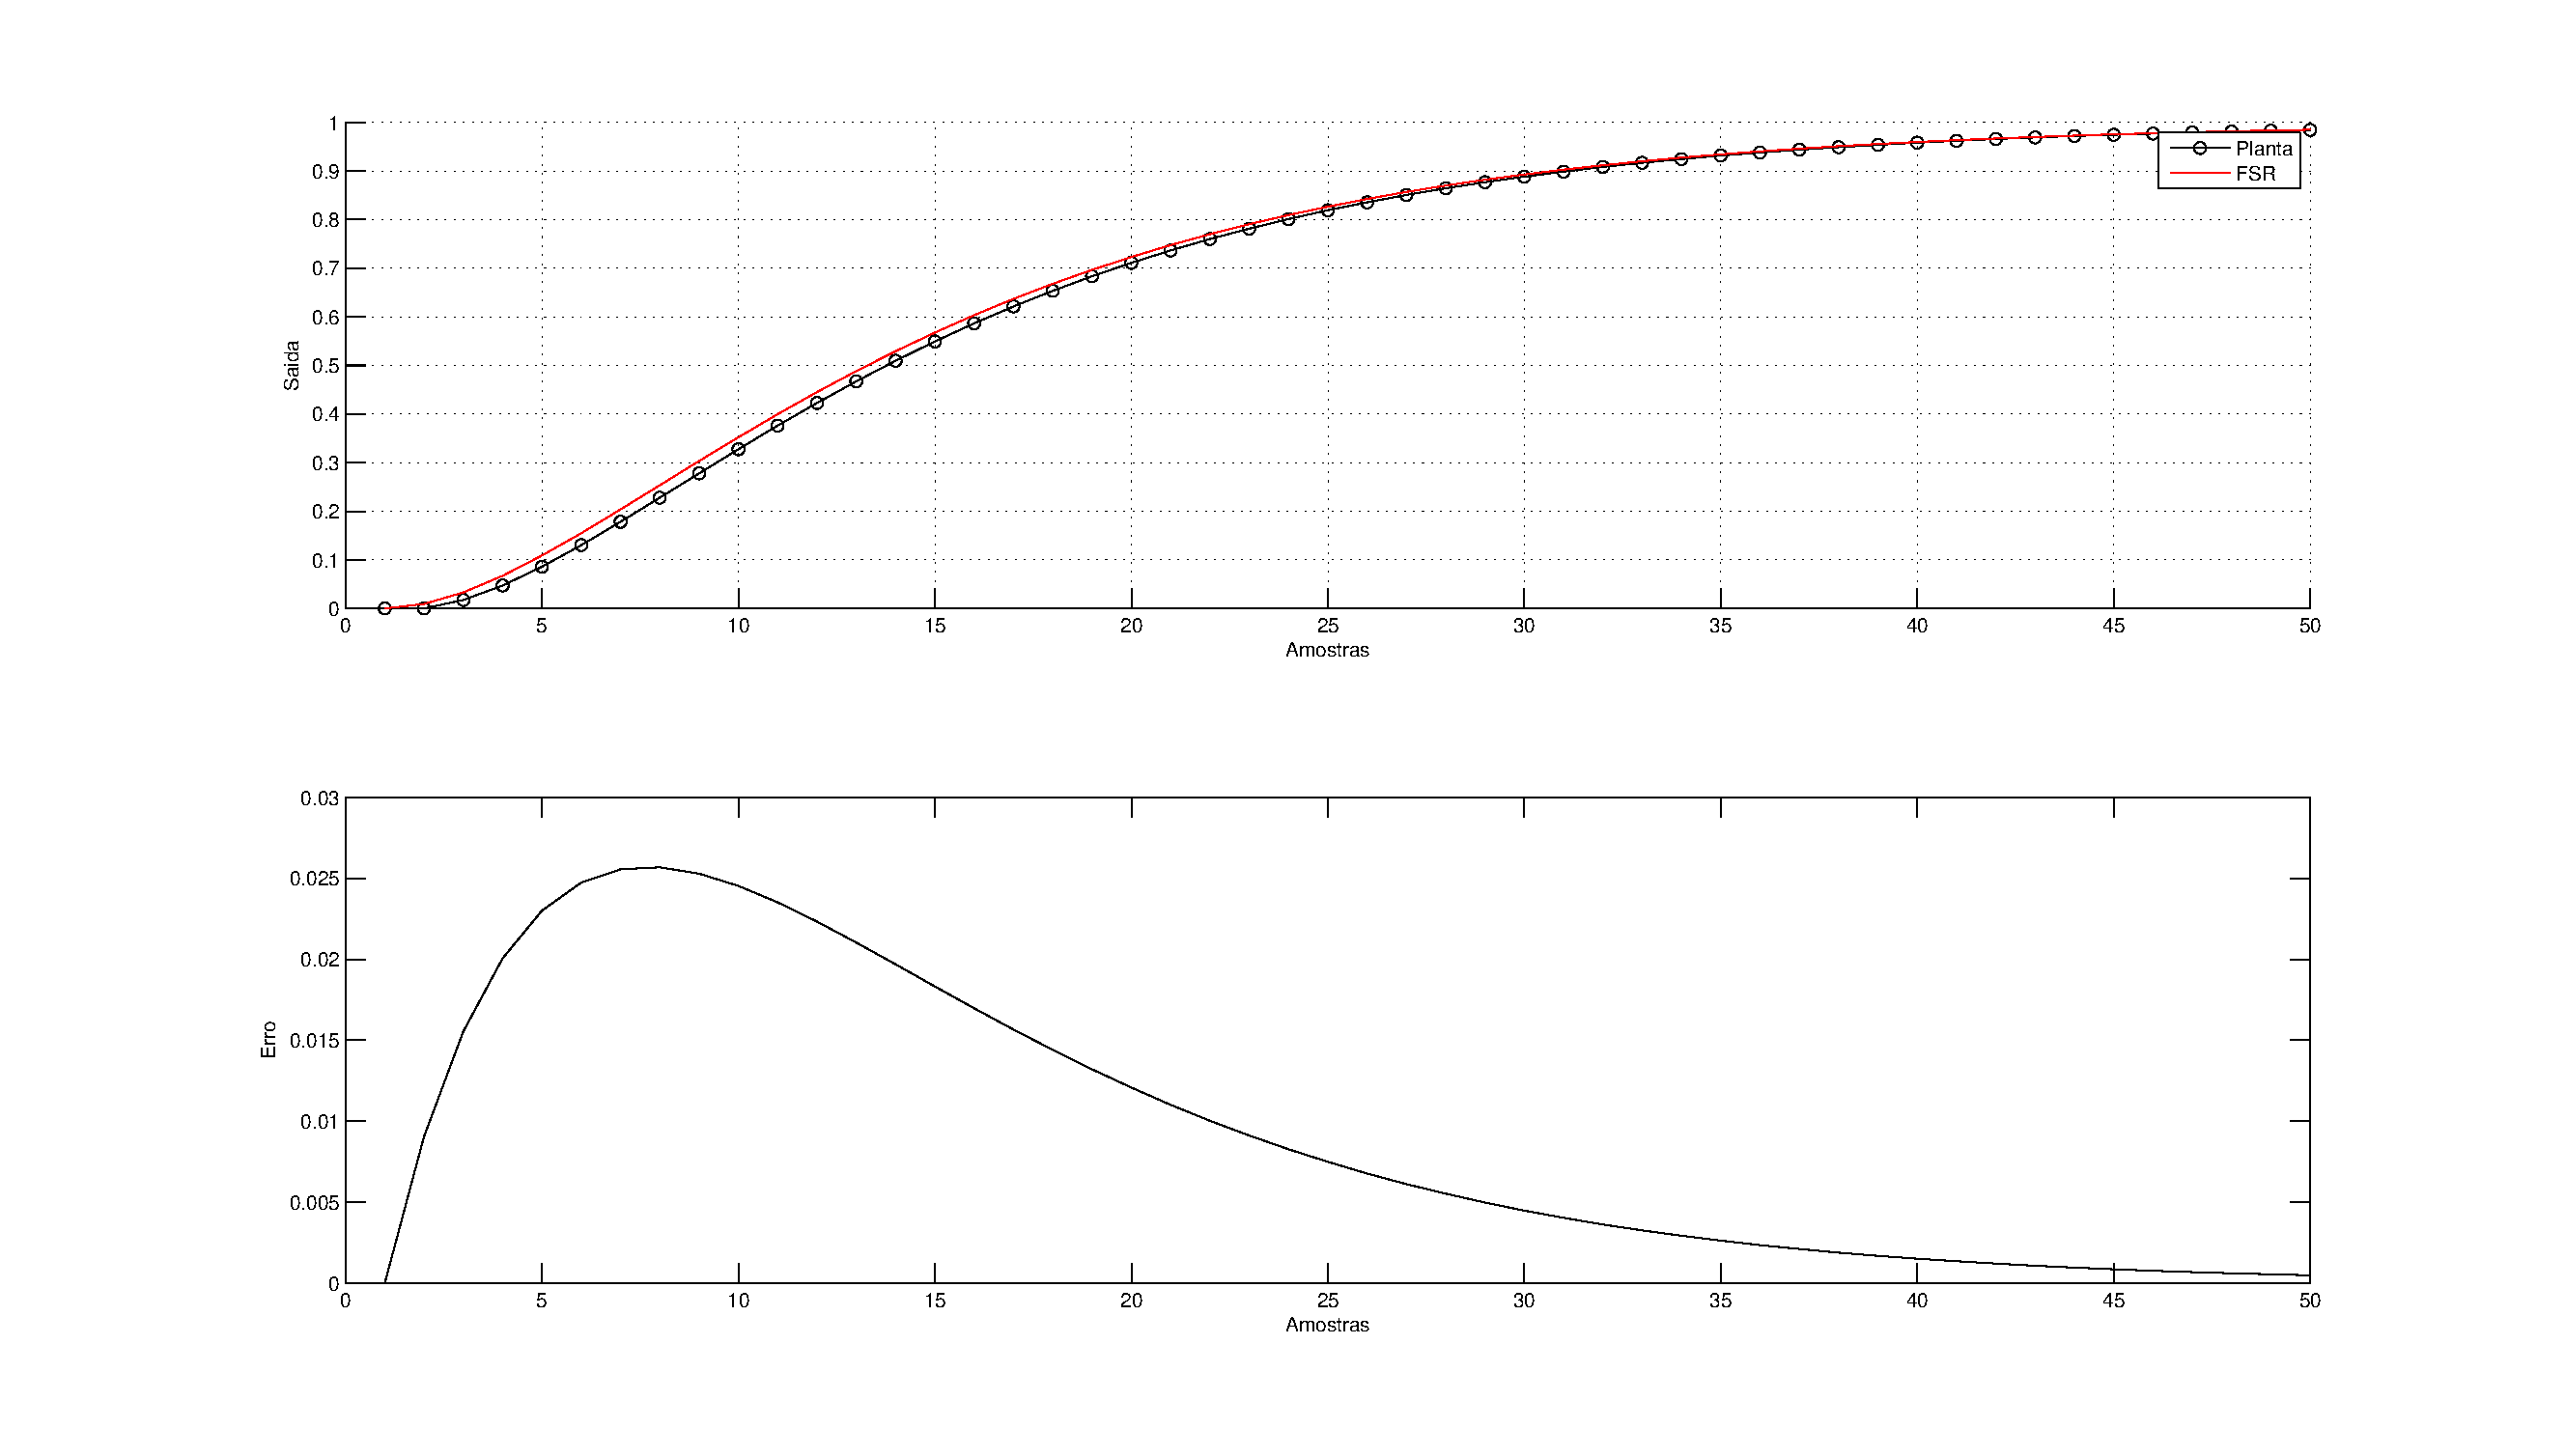
\includegraphics[width=0.95\textwidth]{imgs/questao1/item_c_N_50}
    \caption{Comparação realizada com $N = 50$.}
    \label{fig:item_c_50}
\end{figure}

\begin{figure}[H]
\centering
    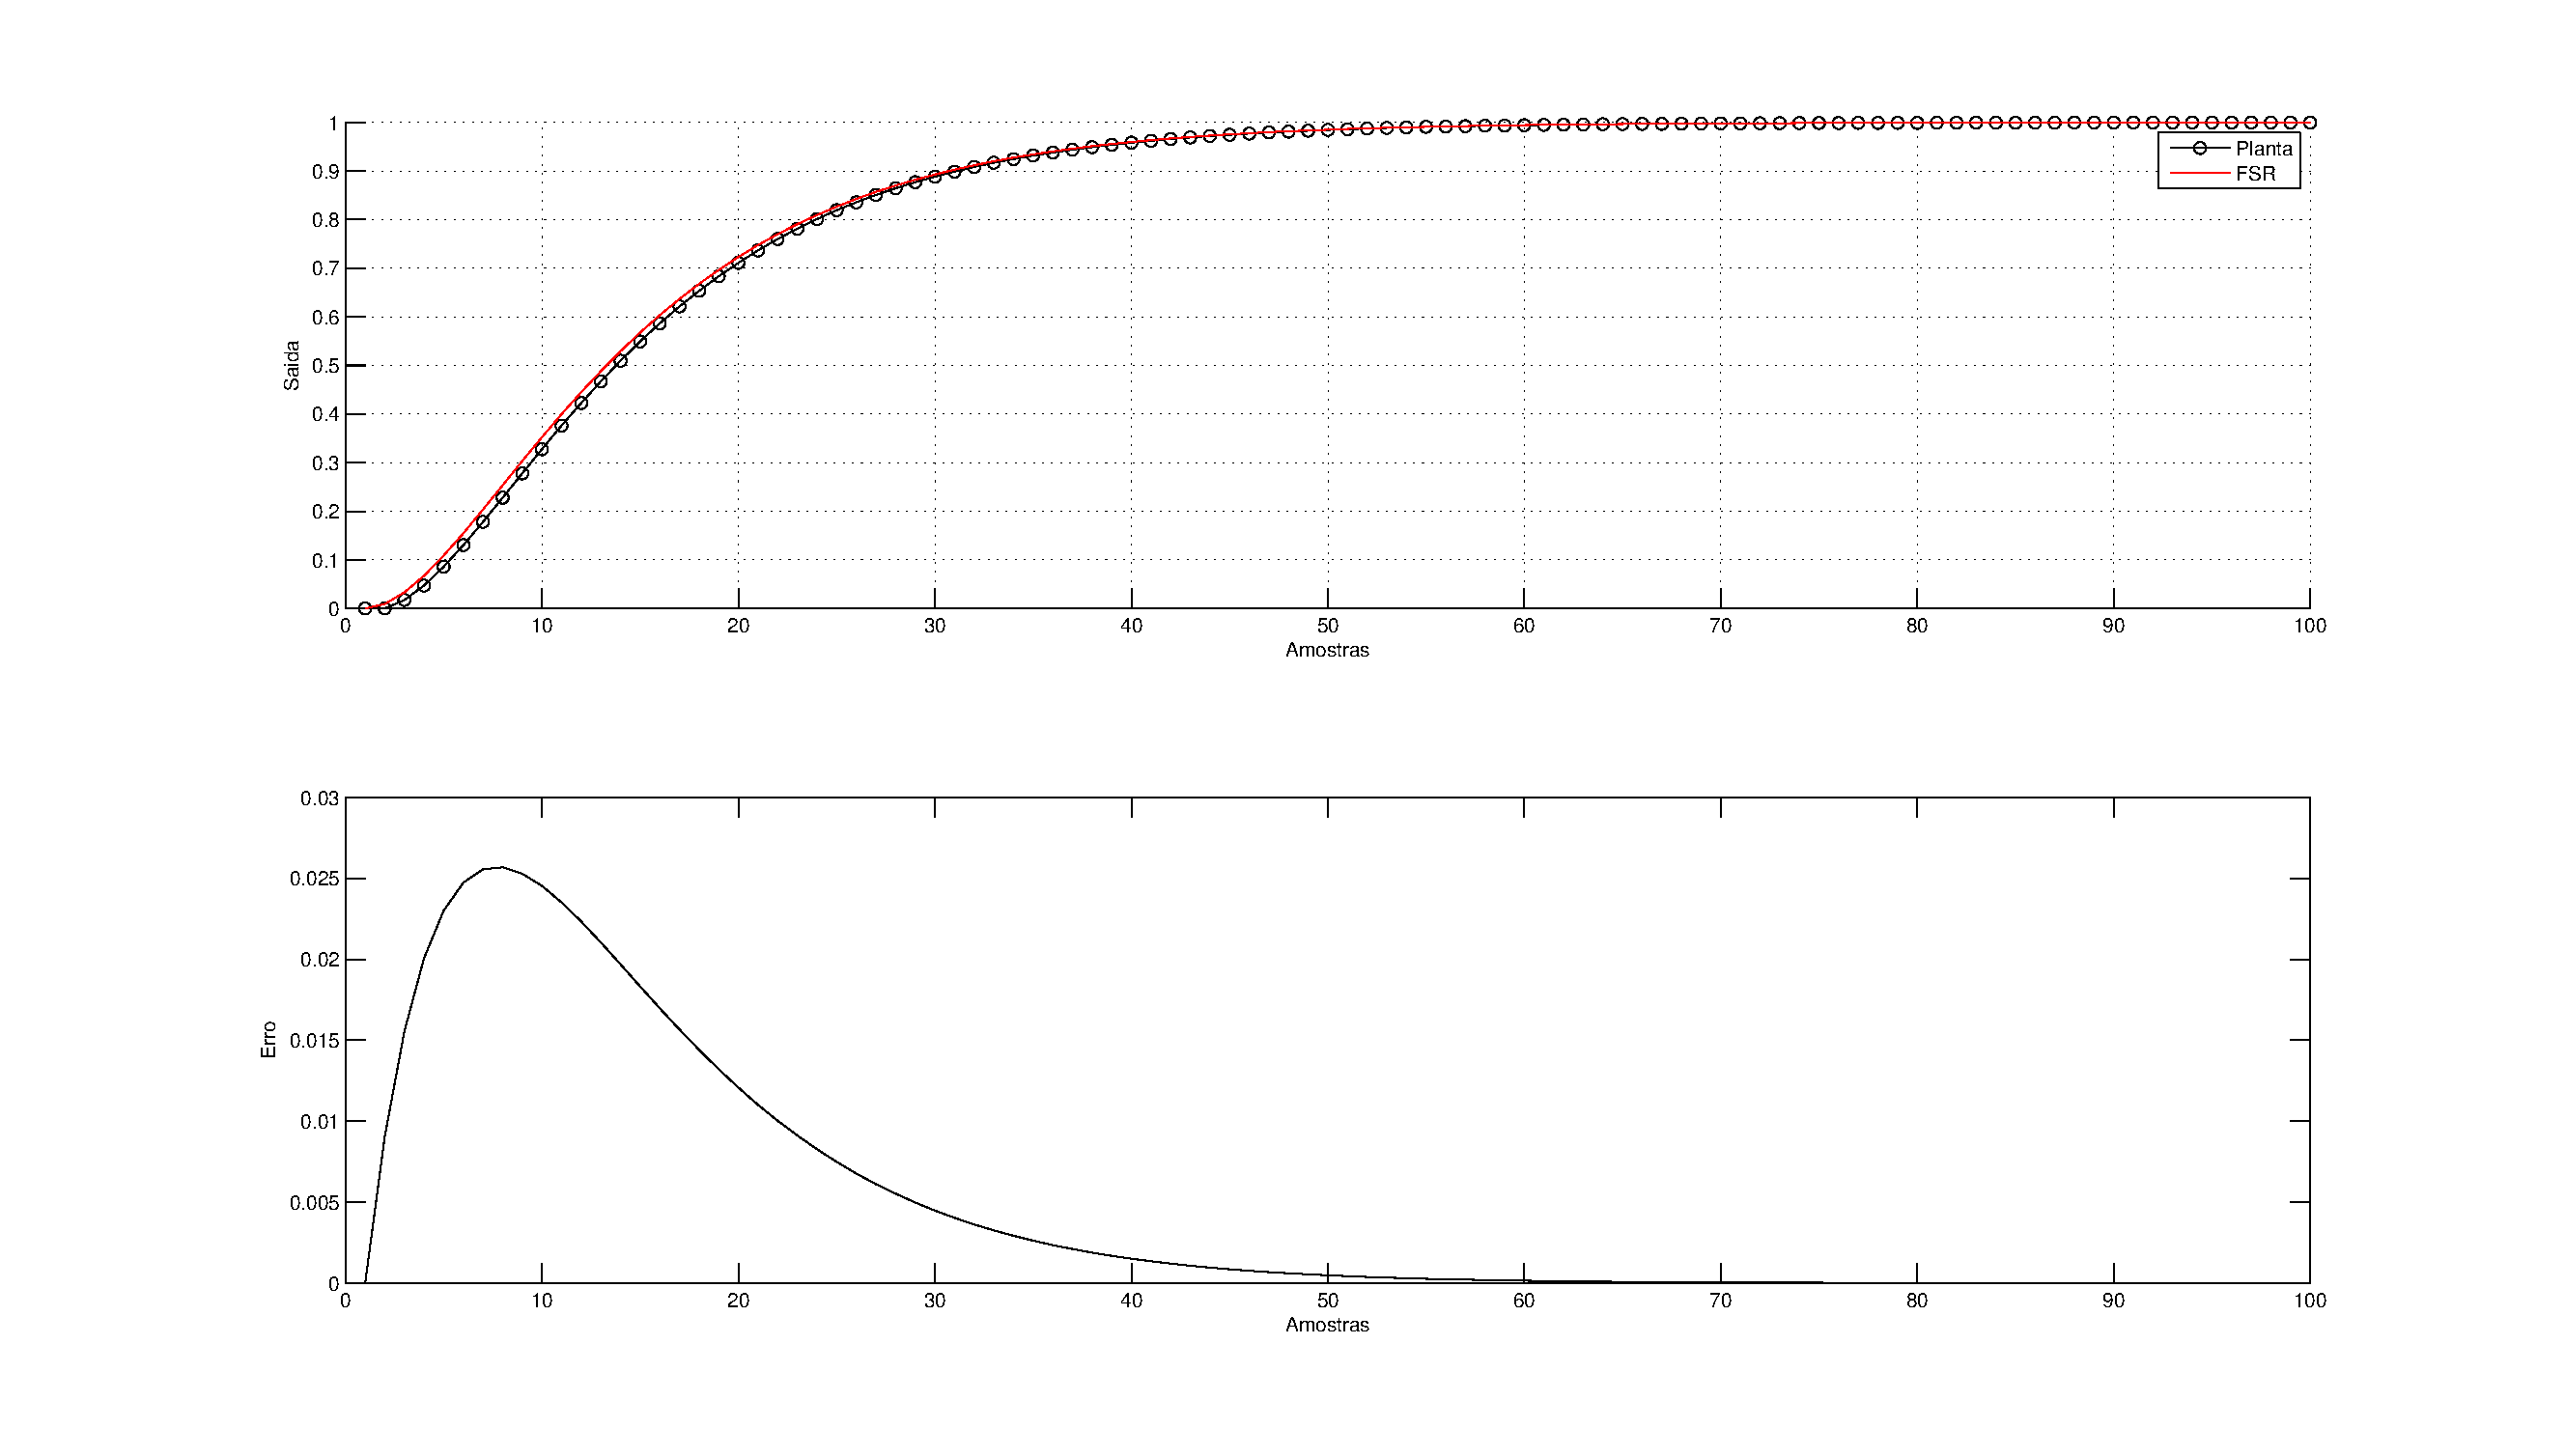
\includegraphics[width=0.95\textwidth]{imgs/questao1/item_c_N_100}
    \caption{Comparação realizada com $N = 100$.}
    \label{fig:item_c_100}
\end{figure}

Observando-se as curvas de erro absoluto, percebe-se que para valores mais
elevados de $N$, ou seja, para um número maior de coeficientes, o sistema
tende a convergir mais rapidamente.

O {\it script} do \Matlab desenvolvido para a resolução dessa questão pode
ser encontrado no Apêndice \ref{ap:q1_c}.

\section*{Item D}
O controlador DMC ({\it Dynamic Matrix Controller}) foi desenvolvido no final da
década de 70 por dois engenheiros da {\it Shell Oil Corporation}. O algoritmo,
desenvolvido em 1979 de maneira não adaptativa e sem restrições, foi modificado
em 1980 de maneira que permitisse a manipulação de restrições.

Anos depois foram propostas diversas modificações para esse algoritmo ao longo
dos anos de maneira a melhorar suas características. Dentre elas, pode-se citar
as implementações com tratamento de restrições e através de espaço de estados.
O sucesso do algoritmo hoje se deve também aos produtos comerciais desenvolvidos
que possuem funcionalidades como a identificação de modelos e a otimização
global de plantas.

Esse controlador utiliza o modelo de {\it resposta ao degrau truncada} (FSR),
fazendo uso de diversos parâmetros com o intuito de garantir uma boa qualidade
de predição. O erro de predição do controlador é considerado como sendo um
distúrbio atuante na saída.

Para o caso monovariável sem restrições, considera-se uma planta, estável em
malha aberta, cuja resposta ao degrau pode ser descrita através de infinitos
coeficientes:

\begin{equation}\label{eq:fsr_inf}
y(k) = \sum_{i=1}^\infty h_i\Delta u(k-i)
\end{equation}

Na prática, utiliza-se um modelo de resposta truncada, conforme Eq.
\ref{eq:saida_fsr}, introduzindo-se a variável erro (usualmente inferior a 5\%):

\begin{equation}\label{eq:fsr_erro}
y(k) = \sum_{i=1}^N h_i\Delta u(k-i) + e(k)
\end{equation}

Baseado no modelo descrito pela Eq. \ref{eq:fsr_erro}, calcula-se um valor
aproximado para $y(k)$ que será diferente da saída real devido ao erro de
modelagem e a um possível ruído a ser inserido no processo de medição: 

\begin{equation}\label{eq:y_til}
\tilde{y}(k) \approx \sum_{i=1}^N h_i\Delta u(k-i)
\end{equation}

O erro inerente ao truncamento e ao ruído de medição pode ser calculado da
seguinte forma:

\begin{equation}\label{eq:erro}
e(k) = y_m(k) - \tilde{y}(k) = y_m(k) - \sum_{i=1}^N h_i\Delta u(k-i)
\end{equation}

\noindent em que $y_m(k)$ corresponde ao valor que deveria ser medido na saída
no instante $k$. Assim sendo, para o instante $k+j$, tem-se:

\begin{eqnarray}
\tilde{y}(k+j) & = & \sum_{i=1}^N h_i\Delta u(k+j-i) + \tilde{e}(k+j)\nonumber\\
\tilde{y}(k+j) & = & \sum_{i=1}^j h_i\Delta u(k+j-i) +
                     \sum_{i=j+1}^N h_i\Delta u(k+j-i) + \tilde{e}(k+j)\nonumber
\end{eqnarray}

Uma vez que não é possível estimar o valor futuro do erro de predição a partir
do modelo, intrinsecamente determinístico, o algoritmo supõe que os erros das
$j$-ésimas predições à frente serão iguais ao erro calculado no instante atual:

\begin{equation}\label{eq:y_pred}
\tilde{y}(k+j) = \sum_{i=1}^j h_i\Delta u(k+j-i) +
                 \sum_{i=j+1}^N h_i\Delta u(k+j-i) + e(k)
\end{equation}

Substituindo a Eq. \ref{eq:erro} na Eq. \ref{eq:y_pred}, tem-se:

\begin{equation}\label{eq:dmc}
\tilde{y}(k+j) = \underbrace{\sum_{i=1}^j h_i\Delta u(k+j-i)}_
                 {\text{parcela forçada}} +
                 \underbrace{\sum_{i=j+1}^N h_i\Delta u(k+j-i) +
                             y_m(k) - \sum_{i=1}^N h_i\Delta u(k-i)}_
                 {\text{parcela livre}}
\end{equation}

O primeiro termo, que corresponde a {\it parcela forçada} ($\tilde{y}_f$), pode
ser obtido considerando-se condições iniciais nulas (em $k$) e a sequência das
ações de controle futuras. Os dois outros termos, correspondentes a {\it parcela
livre} ($\tilde{y}_l$), são obtidos a partir da resposta natural do sistema, com
as condições atuais, considerando a sequência de ações de controle futuras
iguais a zero.

Para a resposta livre, tem-se que:

\begin{equation*}
\tilde{y}_l(k+j) = \sum_{i=j+1}^N h_i\Delta u(k+j-i) + y_m(k) - 
                   \sum_{i=1}^N h_i\Delta u(k-i)
\end{equation*}

Rearranjando os termos quando $N \rightarrow \infty$, tem-se:

\begin{equation}\label{eq:resp_livre}
\tilde{y}_l(k+j) = y_m(k) + \sum_{i=1}^\infty (h_{j+i}-h_i)\Delta u(k-i)
\end{equation}

Se o sistema for assintoticamente estável, após $N$ períodos de amostragem,
tem-se:

\begin{equation*}
h_{j+i} - h_i \approx 0
\end{equation*}

Expandindo então a Eq. \ref{eq:dmc}, tem-se:

\begin{eqnarray}
\tilde{y}(k+1)  & = & h_1\Delta u(k) + h_2\Delta u(k-1) + \ldots + h_N\Delta
                      u(k-N+1) + e(k)\nonumber\\
\tilde{y}(k+2)  & = & h_1\Delta u(k+1) + h_2\Delta u(k) + \ldots + h_N\Delta
                      u(k-N+2) + e(k)\nonumber\\
& \vdots & \nonumber\\
\tilde{y}(k+NY) & = & h_1\Delta u(k+NY-1) + h_2\Delta u(k+NY-2) + \ldots + 
                      h_N\Delta u(k-N+NY) + e(k)\nonumber
\end{eqnarray}

Na qual a resposta livre corresponde as parcelas:

\begin{eqnarray}
\tilde{y}_l(k+1)  & = & h_2\Delta u(k-1) + h_3\Delta u(k-2) + \ldots +
                        h_N\Delta u(k-N+1) + e(k)\nonumber\\
\tilde{y}_l(k+1)  & = & h_3\Delta u(k-1) + h_4\Delta u(k-2) + \ldots +
                        h_N\Delta u(k-N+2) + e(k)\nonumber\\
& \vdots & \nonumber\\
\tilde{y}_l(k+NY) & = & h_{NY+1}\Delta u(k-1) + h_{NY+2}\Delta u(k-2) + 
                        \ldots + h_N\Delta u(k-N+NY) + e(k)\nonumber
\end{eqnarray}

Assim, matricialmente, tem-se:

\begin{equation}\label{eq:resp_livre_mat}
\mb{\tilde{Y}}_l = 
\colchete
{
    \begin{array}{cccc}
        h_N & h_{N-1} & \ldots & h_2\\
        0 & h_N & \ldots & h_3\\
        \vdots & \vdots & \ddots & \vdots\\
        0 & 0 & \ldots & h_N
    \end{array}
}
\colchete
{
    \begin{array}{c}
        \Delta u(k-N+1)\\
        \vdots\\
        \Delta u(k-2)\\
        \Delta u(k-1)
    \end{array}
}
+
\colchete
{
    \begin{array}{c}
        e(k)\\
        e(k)\\
        \vdots\\
        e(k)
    \end{array}
}
\end{equation}

Para a resposta forçada, observa-se que, por definição, $\Delta u(k+i) = 0$,
para $i \geq NU$ ou $i < 0$, sendo $NU$ o horizonte de controle, ou seja, ao
número de incrementos futuros a serem fornecidos à ação de controle atual.
Assim, verifica-se que:

\begin{eqnarray}
\tilde{y}_f(k+1)  & = & h_1\Delta u(k)\nonumber\\
\tilde{y}_f(k+2)  & = & h_1\Delta u(k+1) + h_2\Delta u(k)\nonumber\\
& \vdots & \nonumber\\
\tilde{y}_f(k+NU) & = & h_1\Delta u(k+NU-1) + \ldots + 
                        h_{NU-1}\Delta u(k)\nonumber\\
& \vdots & \nonumber\\
\tilde{y}_f(k+NY) & = & h_{NY-NU}\Delta u(k+NU) + \ldots + 
                        h_{NY}\Delta u(k)\nonumber
\end{eqnarray}

Matricialmente, tem-se:

\begin{equation}\label{eq:resp_forc_mat}
\mb{\tilde{Y}}_f = 
\colchete
{
    \begin{array}{cccc}
        h_1 & 0 & \ldots & 0\\
        h_2 & h_1 & \ldots & 0\\
        \vdots & \vdots & \ddots & \vdots\\
        h_{NY} & h_{NY-1} & \ldots & h_1
    \end{array}
}
\colchete
{
    \begin{array}{c}
        \Delta u(k)\\
        \Delta u(k+1)\\
        \vdots\\
        \Delta u(k+NU)\\
    \end{array}
}
\Rightarrow \mb{\tilde{Y}}_f = \mb{H}\Delta\mb{U}
\end{equation}

A matriz $\mb{H}$ é conhecida como matriz dinâmica, a qual dá origem ao nome do
algoritmo. O valor pretido é então dado por:

\begin{equation}\label{eq:y_pred_mat}
\mb{\tilde{Y}} = \mb{\tilde{Y}}_l + \mb{\tilde{Y}}_f
\mb{\tilde{Y}} = \mb{\tilde{Y}}_l + \mb{H}\Delta\mb{U}
\end{equation}

Vale observar que a matriz $\mb{H}$ é constituída de $NU$ colunas obtidas a
partir da resposta ao degrau do sistema, apropriadamente escolhidas em ordem
decrescente.

Os próximos incrementos da ação de controle são obtidos através do seguinte
critério de minimização:

\begin{equation*}
J = \sum_{j=1}^{NY}\colchete{\hat{y}(k+j)-r(k-j)}^2 + 
    \sum_{j=1}^{NU}\colchete{\lambda\Delta u(k+j)}^2
\end{equation*}

Uma das vantagens da utilização desse critério é que a variação de controle é
considerada, evitando $J$ cresça indefinidamente. Fazendo uso da notação
matricial, tem-se:

\begin{eqnarray}
J & = & \parent{\mb{\tilde{Y}}-\mb{R}}^T\parent{\mb{\tilde{Y}}-\mb{R}} + 
        \lambda\Delta\mb{U}^T\Delta\mb{U}\nonumber\\
& = & \parent{\mb{\tilde{Y}}_l+\mb{H}\Delta\mb{U}-\mb{R}}^T
      \parent{\mb{\tilde{Y}}_l+\mb{H}\Delta\mb{U}-\mb{R}} + 
      \lambda\Delta\mb{U}^T\Delta\mb{U}\nonumber
\end{eqnarray}

Fazendo $\D\frac{\partial J}{\partial\Delta\mb{U}} = 0$, tem-se:

\begin{equation*}
\frac{\partial J}{\partial\Delta\mb{U}} = 
2\mb{H}^T\mb{H}\Delta\mb{U} + 
2\mb{H}^T\parent{\mb{\tilde{Y}}_l-\mb{R}} +
2\lambda\Delta\mb{U} = 0
\end{equation*}

O que leva a:

\begin{equation*}
\parent{2\mb{H}^T\mb{H} + 2\lambda \mb{I}}\Delta\mb{U} = -
2\mb{H}^T\parent{\mb{\tilde{Y}}_l-\mb{R}} \\
\end{equation*}

\begin{equation}\label{eq:delta_u}
\Delta\mb{U} = \parent{\mb{H}^T\mb{H}+\lambda\mb{I}}^{-1}\mb{H}^T
               \parent{\mb{R}-\mb{\tilde{Y}}_l}
\end{equation}

\section*{Item E}
